\section{Pipeline characteristics}
\subsection*{Number of stages}
\hspace{\parindent}The Cortex-A72 processor has a variable-length pipeline, the minimum length of which is 15 stages. This is a result of the different functional units included in the CPU, and so the maximum pipeline length can vary in other ARMv8-based processors. \cite{pipeline} The A72's pipeline is, for the most part, the same as that of its predecessor, the Cortex-A57.
\subsection*{Names}
\hspace{\parindent}To simplify the the pipeline model, its stages can be divided into 5 groups and named according to the functional units that perform them: \cite{pipeline}
\begin{itemize}
	\item \textbf{Fetch}, during cycles 1-5.
	\item \textbf{Decode}, during cycles 6-12.
	\item \textbf{Issue}, in cycle 13.
	\item \textbf{Execute}, during the following cycles, depending on the required execution units; integer and branch operations take the shortest, at only one cycle.\footnote{This stage is the only significant difference between the Cortex-A72's pipeline and the A57's, whose functional units exhibit deeper pipelines.}
	\item \textbf{Retire}, or commit, in the last cycle.
\end{itemize}
\hspace{\parindent}
\begin{figure}[H]
	\begin{center}
		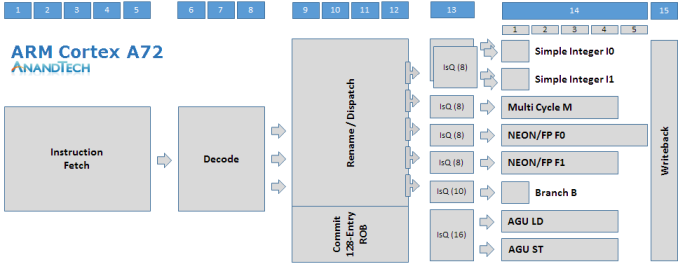
\includegraphics[width=0.7\linewidth]{imgs/a72pipeline.png}
		\caption{The structure of a Cortex-A72 processor core}
	\end{center}
\end{figure}
\pagebreak{}
\section{Steps of instruction execution}
\subsection*{Fetch}
\hspace{\parindent}Instruction execution begins as up to three instructions are fetched from the L1 instruction cache. For branch instructions, prediction also takes place during this stage, making use of the BTB and static predictor this architecture provides.
\subsection*{Decode}
\hspace{\parindent}In this next stage, the previous instructions are decoded into micro-operations to be fed into the execution units, register renaming is performed, removing any potential WAW or WAR hazards, and up to five of the decoded micro-ops are dispatched to the issue queues; this stage could therefore be interpreted as three separate ones (decode, rename and dispatch), with the first taking four cycles, and the latter two taking two cycles each.

Performing register renaming is key in order to facilitate out-of-order execution in the following stages. It should also be noted that, prior to the renaming, the instructions operate on a virtual register pool, which helps to prevent the number of registers specified at the architectural level from becoming a bottleneck. \cite{renaming}
\subsection*{Issue}
\hspace{\parindent}Once they have entered the issue queue, the micro-operations are scheduled onto their respective execution units, up to eight at a time, corresponding to the eight execution units of this processor. From this point on, instruction execution is performed out-of-order.
\subsection*{Execute}
\hspace{\parindent}This stage is different for each instruction, due to the different execution units that perform this step. Here it is worth noting that some of the more common operations (basic integer operations, vector operations, and load/stores, in this case) have two available execution units, in order to avoid structural hazards.
\subsection*{Retire}
\hspace{\parindent}Finally, once all the micro-ops of a given instruction have finished executing, its result is written to a 128-entry re-order buffer, and then sent back to the dispatch unit to update the register files and commit the instructions in order.
\pagebreak{}
\section{Performance studies}
%TODO ask miguel játiva re: content overlap

